The full Promela model, with the LTL properties for the CWP, is in a public Github repository as mentioned previously \cite{repo}. The README.md in the repository summarizing the content and how to reproduce the proof certificate for the model. The actual Promela model is divided into three files: the CWP object state, the CWP LTL properties, and the BPMN workflow model. These are combined with a script to create the final Promela model and verify all twenty properties.

\begin{figure}
  \begin{center}
    \begin{tabular}{c}
      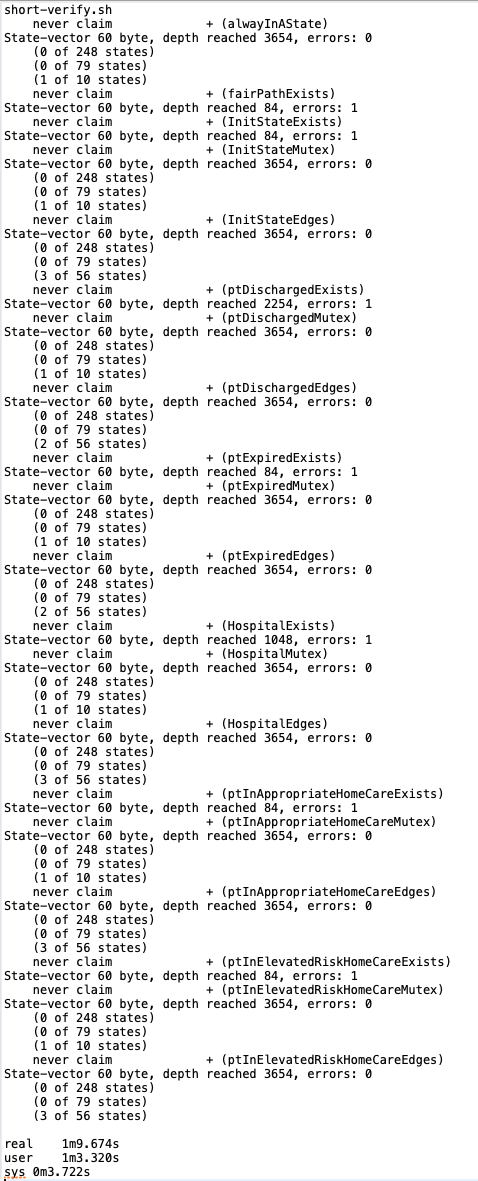
\includegraphics[scale=0.4]{proof.png}
    \end{tabular}
  \end{center}
\caption{The verification results from the SPIN model checker.}
\label{fig:proof}
\end{figure}

The complete verification takes around 3 minutes running on an Intel Core i7 laptop with 16 Gb of RAM. It is not taxing the system significantly. The output from the proof script is shown in \figref{fig:proof}. The output names the property being verified (e.g., the never claim). Following the named property, it summaries the verification effort and what it found. The critical value being the reported errors.

All the existential properties (i.e., the properties ending with \emph{Exists}) should result in an error. The error is the existential witness. All the other properties should pass with no errors. The output of the script includes not just the error report but the coverage summary of the processes and properties. The first two entries pertain to the clinician and patient-caregiver processes. There should never be uncovered states in these processes. The third entry is the property automata being verified. It is not unusual to have uncovered states here when there is no reported error as those states usually correlate with the error state.